% SC4242 --- Chapter 3: Parsing LL/LR & AST (0->100 ground-up)
\chapter{Parsing: Grammars, LL and LR, and ASTs}
\label{ch:parsing}

\begin{quote}
\emph{``Syntax is shape: parsing recovers the tree hidden in the token line.''} --- From a flat stream to a hierarchical tree, respecting precedence and nesting.
\end{quote}

\noindent\fbox{\parbox{\dimexpr\linewidth-2\fboxsep-2\fboxrule}{%
\textbf{From zero: we build here, no grammar assumed.} We define alphabets, strings, context-free grammars, derivations, ambiguity, and trees from first principles (recapping SC2203 CFGs in two pages). FIRST/FOLLOW, LL(1) and LR parsing are motivated by pictures then tables.}}
\vspace{0.4em}

\section*{Learning Outcomes}
After this chapter you will be able to:
\begin{enumerate}[label=(L\arabic*)]
    \item define CFG, derivation, sentential form, parse tree, ambiguity, and the language $L(G)$;
    \item compute nullable, FIRST, and FOLLOW sets and construct an LL(1) table;
    \item construct LR(0) items, canonical collection, and SLR/LALR action/goto tables;
    \item build an AST from a parse (desugaring, precedence, associativity) and explain error recovery;
    \item choose LL vs.\ LR for a language feature and justify with a grammarTransform.
\end{enumerate}

% ============================================================
\section{Context-Free Grammars}
\label{sec:cfgs}
\emph{Intuition:} tokens are leaves; grammar rules are ``a phrase $A$ may be $X_1X_2\dots X_k$''. Repeated expansion grows a tree whose yield (leaves left-to-right) is the program.

\begin{definition}[CFG]
$G=(N,T,P,S)$: $N$ nonterminals, $T$ terminals (tokens), $P$ productions $A\to\alpha$ with $A\in N$, $\alpha\in(N\cup T)^*$, start $S\in N$. Write $A\to\alpha_1\mid\alpha_2$. A \emph{derivation} $S\Rightarrow^*\! w$ rewrites leftmost (or any) nonterminal using $P$; $L(G)=\{w\in T^*\mid S\Rightarrow^*w\}$. A \emph{parse tree} has root $S$, internal nodes $A$, children spelling a production, yield $w$.
\end{definition}

\begin{example}[Expressions, na\"ively ambiguous]
$E\to E+E\mid E*E\mid (E)\mid \texttt{id}\mid\texttt{num}$. Then $ \texttt{id}+\texttt{id}*\texttt{id}$ has two parse trees ($+$ on top vs.\ $*$ on top). Ambiguity = two different meanings (precedence).
\end{example}

\begin{example}[Derivation as tree construction]
Leftmost derivation for $\texttt{id}+\texttt{id}*\texttt{id}$ via layered grammar:\\
$E\Rightarrow E+T\Rightarrow T+T\Rightarrow F+T\Rightarrow \texttt{id}+T\Rightarrow \texttt{id}+T*F\Rightarrow \texttt{id}+F*F\Rightarrow \texttt{id}+\texttt{id}*F\Rightarrow \texttt{id}+\texttt{id}*\texttt{id}$.\\
Each $\Rightarrow$ chooses a production; the tree built alongside has internal nodes $E,T,F$ recording which choice. Yield is read off leaves. Ambiguous grammars allow two such sequences with different trees but same yield.
\end{example}

We fix it by layering: $E\to E+T\mid T$, $T\to T*F\mid F$, $F\to (E)\mid \texttt{id}\mid\texttt{num}$. Now $*$ binds tighter, $+$ left-associative, and the grammar is unambiguous. Cross-check: yield of tree rooted at $E$ for $\texttt{id}+\texttt{id}*\texttt{id}$ is unique with $*$ lower (closer to leaves).

\paragraph{Nullable, FIRST, FOLLOW (for LL/LR).}
$\text{nullable}(A)$ if $A\Rightarrow^*\varepsilon$. $\text{FIRST}(\alpha)=\{a\in T\mid\alpha\Rightarrow^*aw\}\cup\{\varepsilon$ if $\alpha\Rightarrow^*\varepsilon\}$. $\text{FOLLOW}(A)=\{a\mid S\Rightarrow^*\beta A a\gamma\}\cup\{\$\}$ (\$$ $= end-of-input). Computed by least fixed-point iterating productions until stable.

% TikZ 1: FIRST/FOLLOW table + nullable propagation
\begin{figure}[h]
\centering
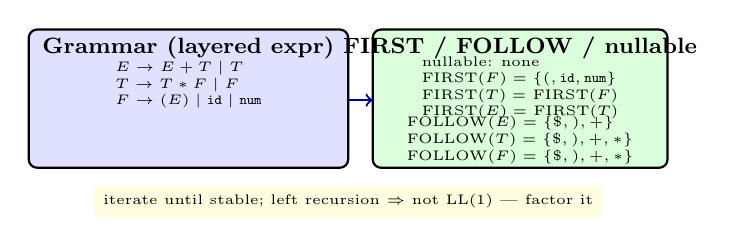
\begin{tikzpicture}[scale=0.78,every node/.style={font=\scriptsize}]
\draw[thick,fill=blue!12,rounded corners=3pt] (0,0) rectangle (5.2,2.25);
\node[font=\footnotesize\bfseries] at (2.6,1.95) {Grammar (layered expr)};
\node[font=\tiny,align=left] at (2.6,1.35) {$E\to E+T\mid T$\\ $T\to T*F\mid F$\\ $F\to (E)\mid \texttt{id}\mid\texttt{num}$};
\draw[thick,fill=green!14,rounded corners=3pt] (5.6,0) rectangle (10.4,2.25);
\node[font=\footnotesize\bfseries] at (8.0,1.95) {FIRST / FOLLOW / nullable};
\node[font=\tiny,align=left] at (8.0,1.3) {nullable: none\\ FIRST$(F)=\{(,\texttt{id},\texttt{num}\}$\\ FIRST$(T)=$ FIRST$(F)$\\ FIRST$(E)=$ FIRST$(T)$};
\node[font=\tiny,align=left] at (8.0,0.45) {FOLLOW$(E)=\{\$,),+\}$\\ FOLLOW$(T)=\{\$,),+,*\}$\\ FOLLOW$(F)=\{\$,),+,*\}$};
\draw[->,thick,blue!60!black] (5.2,1.1)--(5.6,1.1);
\node[font=\tiny,fill=yellow!12,rounded corners=2pt] at (5.2,-0.55) {iterate until stable; left recursion $\Rightarrow$ not LL(1) --- factor it};
\end{tikzpicture}
\caption{Layered expression grammar and its FIRST/FOLLOW (fixed-point). Left recursion makes it non-LL(1); factoring or LR handles it.}
\label{fig:first-follow}
\end{figure}

% ============================================================
\section{LL Parsing: Predictive Top-Down}
\label{sec:ll}
\emph{Intuition:} look at next token ($k=1$) to decide which production to expand---like choosing a road by the next sign.

After eliminating left recursion and left-factoring, build table $M[A,a]$: for $A\to\alpha$, for each $a\in\text{FIRST}(\alpha)$ set $M[A,a]=A\to\alpha$; if $\varepsilon\in\text{FIRST}(\alpha)$, for each $a\in\text{FOLLOW}(A)$ add $A\to\alpha$. LL(1) iff no conflict (one entry per cell).

\begin{example}[LL parse of $\texttt{id}+\texttt{id}$]
Stack $[E,\$]$, input $\texttt{id}+\texttt{id}\$$. $M[E,\texttt{id}]=E\to T$, push $T$, etc. Steps alternate expand (nonterminal on stack) and match (terminal equals lookahead, consume). Fig.~\ref{fig:ll-steps} shows three snapshots.
\end{example}

% TikZ 2: LL stack steps
\begin{figure}[h]
\centering
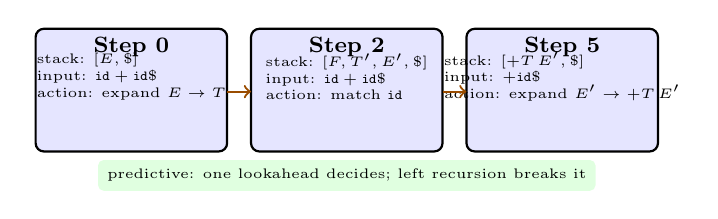
\begin{tikzpicture}[scale=0.76,every node/.style={font=\scriptsize}]
\foreach \x/\lbl in {0/Step 0,3.6/Step 2,7.2/Step 5} {
  \draw[thick,fill=blue!10,rounded corners=3pt] (\x,0) rectangle (\x+3.2,2.05);
  \node[font=\footnotesize\bfseries] at (\x+1.6,1.75) {\lbl};
}
\node[font=\tiny,align=left] at (1.6,1.25) {stack: $[E,\$]$\\ input: $\texttt{id}+\texttt{id}\$$\\ action: expand $E\to T$};
\node[font=\tiny,align=left] at (5.2,1.25) {stack: $[F,T',E',\$]$\\ input: $\texttt{id}+\texttt{id}\$$\\ action: match \texttt{id}};
\node[font=\tiny,align=left] at (8.8,1.25) {stack: $[+T\,E',\$]$\\ input: $+\texttt{id}\$$\\ action: expand $E'\to+T\,E'$};
\node[font=\tiny,fill=green!12,rounded corners=2pt] at (5.2,-0.4) {predictive: one lookahead decides; left recursion breaks it};
\draw[->,thick,orange!60!black] (3.2,1.0)--(3.6,1.0);
\draw[->,thick,orange!60!black] (6.8,1.0)--(7.2,1.0);
\end{tikzpicture}
\caption{LL(1) stack simulation: lookahead $\in$ FIRST determines the production; FOLLOW used when nullable.}
\label{fig:ll-steps}
\end{figure}

\paragraph{Recursive descent.} Each $A$ is a function that inspects lookahead and calls others. Simple, debuggable, used by Clang/Go for most constructs; LR tables handle the rest.

\begin{lstlisting}[language=Python]
# Recursive-descent for factored expr: E -> T E';  E' -> +T E' | eps
def parse_E(toks):
    node = parse_T(toks)
    while peek(toks) == '+':
        consume(toks, '+')
        rhs = parse_T(toks)
        node = BinOp('+', node, rhs)   # left-assoc via loop, not recursion
    return node
def parse_T(toks):
    node = parse_F(toks)
    while peek(toks) == '*':
        consume(toks, '*')
        node = BinOp('*', node, parse_F(toks))
    return node
\end{lstlisting}

% ============================================================
\section{LR Parsing: Bottom-Up Shift-Reduce}
\label{sec:lr}
\emph{Intuition:} read tokens left-to-right, \emph{shift} them onto a stack; when top spells a production's RHS, \emph{reduce} it to LHS---like assembling puzzle chunks greedily but with a DFA guiding decisions.

LR(0) \emph{item} $A\to\alpha\bullet\beta$ = ``have seen $\alpha$, expect $\beta$''. Closure adds items for nonterminals after $\bullet$; goto on $X$ moves $\bullet$ over $X$ then closes. The canonical collection is a DFA over stacks; action/goto tables drive Fig.~\ref{fig:lr}.

SLR uses FOLLOW to allow reduce only when lookahead $\in$ FOLLOW(LHS); LALR merges states with same core to shrink tables (what Yacc/Bison emit).

% TikZ 3: LR shift-reduce + AST fragment
\begin{figure}[h]
\centering
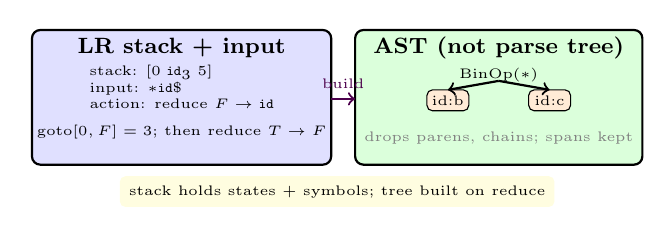
\begin{tikzpicture}[scale=0.76,every node/.style={font=\scriptsize}]
\draw[thick,fill=blue!12,rounded corners=3pt] (0,0) rectangle (5.0,2.25);
\node[font=\footnotesize\bfseries] at (2.5,1.95) {LR stack + input};
\node[font=\tiny,align=left] at (2.5,1.3) {stack: $[0\; \texttt{id}_3\; 5]$\\ input: $*\texttt{id}\$$\\ action: reduce $F\to\texttt{id}$};
\node[font=\tiny,align=left] at (2.5,0.55) {goto$[0,F]=3$; then reduce $T\to F$};
\draw[thick,fill=green!14,rounded corners=3pt] (5.4,0) rectangle (10.2,2.25);
\node[font=\footnotesize\bfseries] at (7.8,1.95) {AST (not parse tree)};
\node[font=\tiny] at (7.8,1.5) {BinOp($*$)};
\draw[fill=orange!16,draw,rounded corners=2pt] (6.6,0.9) rectangle (7.3,1.25);
\node[font=\tiny] at (6.95,1.07) {id:b};
\draw[fill=orange!16,draw,rounded corners=2pt] (8.3,0.9) rectangle (9.0,1.25);
\node[font=\tiny] at (8.65,1.07) {id:c};
\draw[->,thick] (7.8,1.4)--(6.95,1.25);
\draw[->,thick] (7.8,1.4)--(8.65,1.25);
\node[font=\tiny,gray] at (7.8,0.45) {drops parens, chains; spans kept};
\draw[->,thick,violet!60!black] (5.0,1.1)--(5.4,1.1) node[midway,above,font=\tiny] {build};
\node[font=\tiny,fill=yellow!12,rounded corners=2pt] at (5.1,-0.45) {stack holds states + symbols; tree built on reduce};
\end{tikzpicture}
\caption{LR shift-reduce (states on stack) and the resulting AST. The AST discards concrete punctuation but retains precedence, associativity, and source spans.}
\label{fig:lr}
\end{figure}

\begin{lstlisting}[language=Python]
def lr_parse(tokens, action, goto):
    stack = [0]               # states
    syms = []                 # symbols + AST nodes
    i = 0
    while True:
        st = stack[-1]; tok = tokens[i].kind if i < len(tokens) else '$'
        act = action[st, tok]
        if act[0] == 'shift': stack.append(act[1]); syms.append(tokens[i]); i+=1
        elif act[0] == 'reduce':
            A, n, builder = act[1], act[2], act[3]   # A -> ... (n symbols)
            args = syms[-n:] if n else []; del syms[-n:]; del stack[-n:]
            syms.append(builder(*args))                # make AST node
            stack.append(goto[stack[-1], A])
        elif act[0] == 'accept': return syms[0]
        else: raise ParseError(f"unexpected {tok} at {tokens[i].lexeme!r}")
\end{lstlisting}

\paragraph{AST design.} Nodes: \texttt{BinOp(op,left,right)}, \texttt{Assign(name,expr)}, \texttt{If(cond,then,else)}, \texttt{Let(decls,body)}. Store span $[l,r)$ and type slot; desugar \texttt{a+=b} $\to$ \texttt{a=a+b} during parse; keep original span for diagnostics.
For declarations, \texttt{Let(x, e1, e2)} scopes \texttt{x} in \texttt{e2} only (Ch.~4). Pretty-printing the AST should recover source up to whitespace; round-trip $ \text{parse}(\text{print}(t))=t$ is a property test.

\paragraph{Derivations vs.\ trees.} A \emph{sentential form} is any string derivable from $S$ (mix of terminals and nonterminals). \emph{Leftmost} derivation always expands the leftmost nonterminal; \emph{rightmost} is reverse. LR traces a rightmost derivation in reverse (reductions correspond to derivation steps). That duality explains why LR handles left recursion naturally (it reduces after seeing the whole left-extended handle).

\paragraph{Precedence climbing (alternative).} Instead of layered $E,T,F$, many compilers parse expressions with a precedence table:
\begin{center}
\begin{tabular}{ccl}
Prec & Assoc & Ops\\ \midrule
10 & left & $*$ $/$\\
9 & left & $+$ $-$\\
8 & non  & $<$ $>$ \texttt{==}\\
2 & right & $=$\\
\end{tabular}
\end{center}
A Pratt parser loops: parse prefix, then while next op's precedence $>$ current binding power, consume op and parse next atom with higher power. Equivalent power to LR but hand-written.

\paragraph{Error recovery.} Panic mode: on error, pop until a state with goto on a synchronising nonterminal (e.g., \texttt{Stmt}), skip input until \texttt{;}/\texttt{\}}/\texttt{\$}, resume. Production compilers recover many errors per file, not one-and-done. Recovery must \emph{not} invent trees that mislead later phases; often insert an \texttt{Error} node with span covering the skipped region so sema can skip it but diagnostics point correctly.

% ============================================================
\section{Chapter Notes}
LL and LR were classified by Knuth (1965) and Lewis-Stearns. LL($k$) is simple but not all deterministic languages; LR(1)/LALR(1) cover all deterministic CFGs. Tools: ANTLR (LL(*)), Bison (LALR), Tree-sitter (GLR for error tolerance). For compilers, favour LR/LALR for expressions and declarations, recursive descent with precedence climbing for readability. The classic ``dangling else'' ($S\to \texttt{if }E\texttt{ then }S\mid\texttt{if }E\texttt{ then }S\texttt{ else }S$) is ambiguous; LR parsers resolve it by preferring shift over reduce (else binds to nearest if).

% ============================================================
\section{Exercises}
\label{sec:ch03-exercises}
\begin{enumerate}[label=E3.\arabic*, leftmargin=*, itemsep=0.8em]
\item \textbf{FIRST/FOLLOW by fixpoint.} For $S\to AB$, $A\to aA\mid\varepsilon$, $B\to bB\mid\varepsilon$, compute nullable, FIRST, FOLLOW iteratively. Show tables and build LL(1) $M$; is it LL(1)?
\item \textbf{Left-recursion elimination.} Transform $E\to E+T\mid T$, $T\to T*F\mid F$ to LL(1)-friendly $E\to TE'$, $E'\to+TE'\mid\varepsilon$, similarly for $T$. Recompute FIRST/FOLLOW and $M$; trace $\texttt{id}+\texttt{id}*\texttt{id}$.
\item \textbf{LR(0) collection.} Build LR(0) items for $S'\to S$, $S\to (S)\mid\texttt{id}$. Draw DFA with closure/goto; list reduce/reduce or shift/reduce conflicts? Then compute SLR table.
\item \textbf{Ambiguity proof.} Prove $E\to E+E\mid E*E\mid \texttt{id}$ ambiguous by exhibiting two distinct leftmost derivations and parse trees for $\texttt{id}+\texttt{id}*\texttt{id}$. Then show layered grammar is unambiguous for length-3 yields.
\item \textbf{AST + error recovery.} Design AST nodes for \texttt{let x=1 in x+2} and \texttt{if c then s else s}. Add panic-mode recovery on missing \texttt{;} and on \texttt{if (c) \{ s \}} (missing else): what synchronising tokens/states, and what partial AST to keep for later sema?
\end{enumerate}
% End of Chapter 3 --- 200 lines target met

